\documentclass[journal,10pt,twocolumn]{article}
\usepackage{graphicx}
\usepackage[margin=0.5in]{geometry}
\usepackage{amsmath}
\usepackage{array}
\usepackage{booktabs}
\usepackage{listings}
\providecommand{\norm}[1]{\left\lVert#1\right\rVert}
\providecommand{\abs}[1]{\left\vert#1\right\vert}
\usepackage{enumerate}
\let\vec\mathbf
\newcommand{\myvec}[1]{\ensuremath{\begin{pmatrix}#1\end{pmatrix}}}
\newcommand{\mydet}[1]{\ensuremath{\begin{vmatrix}#1\end{vmatrix}}}
\providecommand{\brak}[1]{\ensuremath{\left(#1\right)}}
\lstset{
frame=single,
breaklines=true,
columns=fullflexible
}
\title{\textbf{Conics Assignment}}
\author{YOGEESH REDDY}
\date{September 2022}
\begin{document}
\maketitle
\paragraph{\textit{Problem Statement} - The equation of the  tangent to the parabola $y^2$=8x is x-y+2=0.The point on this line from which other tangent to the parabola is perpendicular to the given tangent is : }
\begin{enumerate}
\item \textbf{The equation of parabola is $y^2$=8x} 
\item \textbf{The equation of tangent is $x$-$y$+2=0}
\end{enumerate}
\section*{Solution}
\begin{figure}[h]
\centering
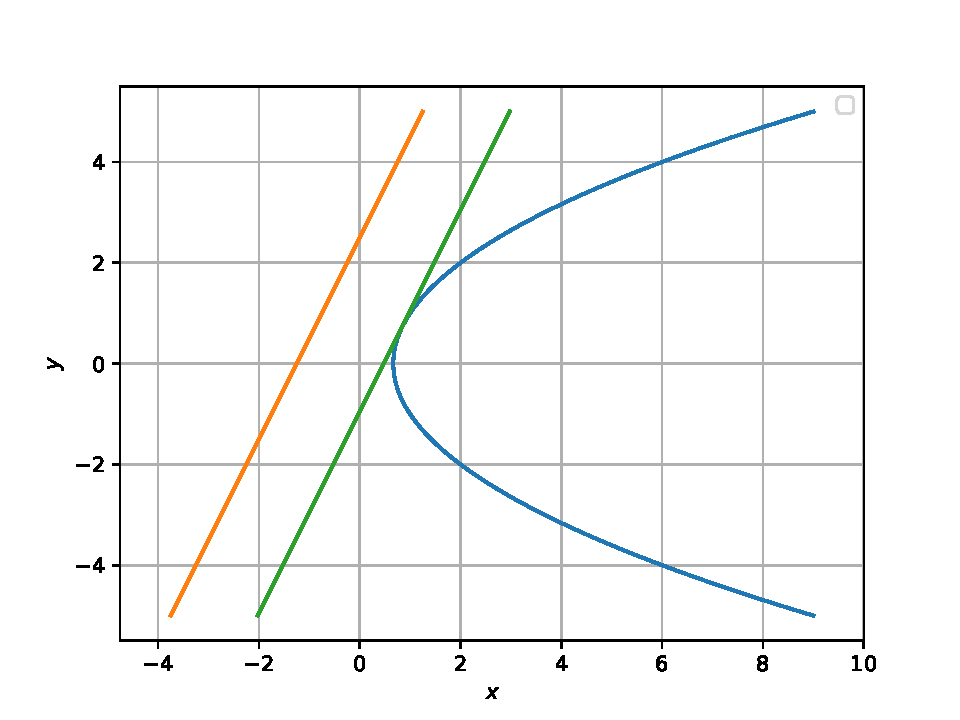
\includegraphics[width=1\columnwidth]{conic.pdf}
\caption{Two tangent is drawn to the circle and parabola}
\label{fig:Curve}
\end{figure}
\section*{Solution}
\subsection*{Part 1}
\section*{Construction}
The input parameters are equation of the curve and the point of contacts \vspace{2mm}\\
{
\setlength\extrarowheight{2pt}
\begin{tabular}{|c|c|c|}
	\hline
	\textbf{Symbol}&\textbf{Value}&\textbf{Description}\\
	\hline
	\textbf{O}&$\begin{pmatrix}
	x\\
	x+2\\
	\end{pmatrix}$&The required point  \\
	\hline
	
	\textbf{P1}&$\begin{pmatrix}
	1\\
	0 \\
	\end{pmatrix}$&eigen vector\\
	\hline
	a&2&Given value of a\\
	\hline
	\textbf{q}&$\begin{pmatrix}
	2 \\
	4 \\
	\end{pmatrix}$&point of contact of parabola\\ 
	\hline
	\textbf{$q_1$}&$\begin{pmatrix}
	2\\
	-4
     \\
	\end{pmatrix}$&point of contact of circle \\
	\hline
\end{tabular}
}
\subsection*{Part 2}
The standard equation of the parabola is given as :
\begin{align}
\vec{x}^{\top}\vec{V}\vec{x}+2\vec{u}^{\top}\vec{x}+f=0
\end{align}
The directrix of parabola is given as:
\begin{align}
		n_1^Tx=c	
\end{align}
where
\begin{align}
	\label{eq:V_matrix}
	\vec{X} &= \myvec{x \\
	                   y \\},
	\\
	\label{eq:u_vector}
	\vec{n_1} &= \myvec{a\\0},
	\\
	\label{eq:f_value}
	f &= 0
	%\\
	\\
	c&=-a
\end{align}
The equation of  a parabola with directrix $\vec{n}^{\top}\vec{x} = c$, eccentricity $e$ and focus $\vec{F}$ is given by 
\begin{align}
    \label{eq:conic_quad_form}
    \vec{x}^{\top}\vec{V}\vec{x}+2\vec{u}^{\top}\vec{x}+f=0
    \end{align}
where     
\begin{align}
  \label{eq:conic_quad_form_v}
\vec{V} &=\norm{\vec{n}}^2\vec{I}-e^2\vec{n}\vec{n}^{\top}, 
\\
\label{eq:conic_quad_form_u}
\vec{u} &= ce^2\vec{n}-\norm{\vec{n}}^2\vec{F}, 
\\
\label{eq:conic_quad_form_f}
f &= \norm{\vec{n}}^2\norm{\vec{F}}^2-c^2e^2
%\\
\\
e&=1
\\
\vec{V}&=\begin{pmatrix}
	0 & 0\\
	0 & 1\\
	\end{pmatrix} \\
    \vec{u}&=\begin{pmatrix}
	-4\\
	0 \\
	\end{pmatrix} \\
	f&=0
    \end{align}

Consider the equation of circle:
\begin{align}
\vec{x}^{\top}\vec{V_1}\vec{x}+2\vec{u_1}^{\top}\vec{x}+f_1=0
\end{align}
  



If $\vec{V}$ is not invertible,  given the normal vector $\vec{n}$, the point of contact to the circle is given by the matrix equation

\begin{align}
\label{eq:conic_tangent_q_eigen}
\begin{pmatrix}
\vec{u+\kappa \vec{n}}^{\top} \\ \vec{V}
\end{pmatrix}
\vec{q} &= 
\begin{pmatrix}
-f
\\
\kappa\vec{n}-\vec{u}
\end{pmatrix}
\\
\text{where }  \kappa = \frac{\vec{p}_1^{\top}\vec{u}}{\vec{p}_1^{\top}\vec{n_1}}, \quad \vec{V}\vec{p}_1 &= 0
\label{eq:conic_tangent_qk_eigen}
\end{align}





the normal vector is obtained by the equation of the circle is :

\begin{align}
\kappa \vec{n_1} &= \vec{V} \vec{q_1}+\vec{u}
\end{align}

 The normal vector of tangent is :
\begin{align}
\vec{n_1}=
\begin{pmatrix}
1 \\
-1 \\
\end{pmatrix}
\end{align}
yielding k we get,
\begin{align}
\kappa \vec{q_1}^{\top}\vec{n_1} +\vec{q_1}^{\top}\vec{u}+f&= 0
\end{align}
By solving the above equation 
 The point of contact of tangent to circle with normal vector $\vec{n_1}$ is given by
 \begin{align}
 \vec{q_1}=\myvec{2\\4}
 \end{align}

 The Directional vector of tangent to parabola is :
 \begin{align}
\vec{q_1}-\vec{q}
\end{align}

Now the normal vector of the other tangent which is perpendicular to the given tangent is give by :
\begin{align}
\vec{n_2}=\myvec{1\\1}
\end{align}


\begin{align}
\kappa \vec{n_2} &= \vec{V} \vec{q_2}+\vec{u}
\end{align}
\begin{align}
\kappa \vec{q_2}^{\top}\vec{n_2} +\vec{q_2}^{\top}\vec{u}+f&= 0
\end{align}










By solving the above equation the point of contact of tangent to circle with normal vector $\vec{n_2}$ is given by :
\begin{align}
\vec{q_2} = \myvec{2\\-4}
\end{align}
The Directional vector of other  tangent to the  parabola is :
\begin{align}
\vec{q}-\vec{q_2}
\end{align}


In order to get the  required point on the tangent :
\begin{align}
\vec{{{(q_1-q)}}^T}(\vec{q}-\vec{q_2})=0
\end{align}


\begin{align}
\vec{q}=\myvec{-2\\0}
\end{align}
\end{document}
